\documentclass{beamer}

\usepackage{amsmath, amssymb}
%\usepackage[utf8]{inputenc}
\usepackage{zxjatype}
\usepackage[ipa]{zxjafont}
\usepackage{mymacro}
\usepackage{graphicx}
\usepackage{caption}
\usepackage{subcaption}
\usepackage{listings}
\usepackage[para,online,flushleft]{threeparttable}

\usefonttheme{professionalfonts}
\setbeamertemplate{navigation symbols}{}

% --- page number ---
\setbeamertemplate{footline}{%
	\raisebox{10pt}{\makebox[\paperwidth]{\hfill\makebox[7em]{\normalsize\texttt{\insertframenumber/\inserttotalframenumber}}}}%
}

\title{Understanding the OKC Rental Market through Analysis of Craigslist Data}
\author{Karley Nadolski}
\date{April 29, 2021}

\begin{document}

    \begin{frame}[plain]
        \maketitle
    \end{frame}

\begin{frame}{Introductions - Craigslist as a Data Source}
       \begin{tabular}{cl}  
         \begin{tabular}{c}
           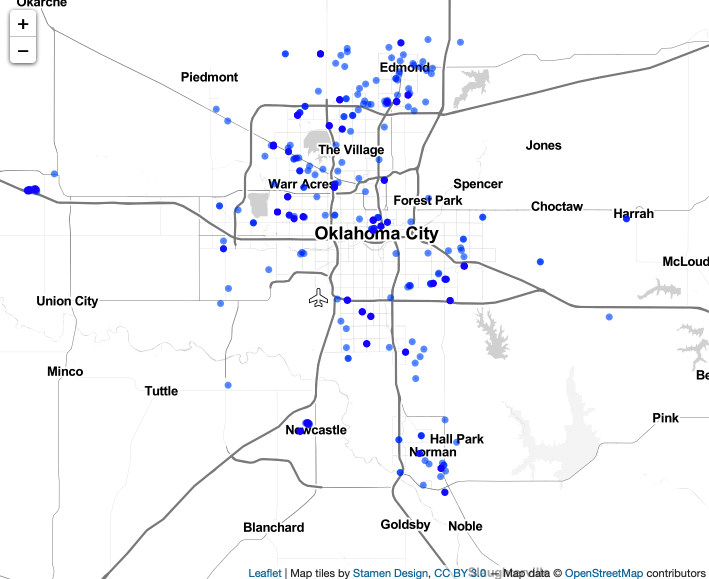
\includegraphics[height=3.5cm, width=4.5cm]{craigslist.mapfar.png}
           \caption{Map of the OKC Metro Area dotted with Craigslist Listings}
           \end{tabular}
           & \begin{tabular}{l}
             \parbox{0.5\linewidth}{%  change the parbox width as appropiate
             \textbf{Craigslist is an important data source for rental markets all over the country}  
     
      Each Craigslist listing is required to include:       
        \begin{itemize}
            \item advertised rent price
            \item user-generated description of the unit
            \item Optional: square footage, number of bedrooms/bathrooms, and other  descriptions about amenities 
        \end{itemize}
    }
         \end{tabular}  \\
         \end{tabular}
\end{frame}

\begin{frame}[plain,c]
        \begin{center}
            \Large Does the extra information in Craigslist descriptions matter? What's the premium of extra information in the Craigslist rental market?
        \end{center}
\end{frame}

\begin{frame}[fragile]{Data Collection - Webscraping}
        \begin{itemize}
            \item Step 1: fill out baseurl ("https://oklahomacity.craigslist.org/search/apa")
            \item Step 2: build queries (bedrooms=2, bathrooms=1, sqft=900)
            \item Step 3: choose which attributes to extract from each listing (ID, title, price, sqft, etc...)
            \item Step 4: coerce code into a for loop to iterate through all listings within the query
            \item Step 5: organize and clean data
        \end{itemize}
\end{frame}

\begin{frame}[fragile]{Methods}
    \begin{equation}
    Y_{price}=\left(\begin{tabular} {l}
    \beta_{0} + \beta_{1}X_{sqft} + \beta_{2} X_{bdrms} + \beta_{3}X_{p.QDAP} + \beta_{4}X_{wordcount} \\ + \beta_{5}X_{t.wordcount}+\beta_{6}X_{t.direction} + \varepsilon,
    \end{tabular}\right)
    \end{equation}
    
    where $Y_{price}$ is a continuous variable describing the price of each rental listing, $X_{sqft}$ is the square footage of the rental unit, $X_{bdrms}$ is the number of bedrooms, $X_{p.QDAP}$ is the positivity index from the listing's description, $X_{wordcount}$ and $X_{t.wordcount}$ are the word counts for the description and the title, respectively, and finally $X_{t.direction}$ describes the sentiment of the listing title.
\end{frame}

\begin{frame}[plain,c]
        \begin{center}
            \Large Research Findings
        \end{center}
\end{frame}

\begin{frame}{Findings}

\begin{table}[ht]
\caption{OLS estimates}
\centering
\begin{threeparttable}
\begin{tabular}{lccc}
\toprule
                            & Estimate    & Std. Error & P-value \\
\midrule
sqft        & 0.89505***   & (0.03317)    & $<2e-16$    \\
bdrms  & -234.539***   & (18.02865)   & $<2e-16$ \\
p.QDAP        &      229.54856 & (184.04089)  & 0.21255 \\
wordcount     &    1.87407***  & (0.10400)    & $<2e-16$\\
t.wordcount & -12.57888**  & (4.26128) & 0.00322 \\
t.directionneutral & 86.17754* & (41.89659) & 0.03992 \\
t.directionpositive & 100.19908* & (41.44415) & 0.01577 \\
\bottomrule
\end{tabular}
\footnotesize Notes: Standard errors in parentheses. ***Significantly different from zero at the .1\% level; **Significantly different from zero at the 1\% level. *Significantly different from zero at the 5\% level. 
\end{threeparttable}
\end{table}

\end{frame}

\begin{frame}{What did we learn? Why was it important? }
    \begin{itemize}
        \item For every additional word in a unit description, the rental price rises by about \$2 per month
        \item For every additional word in a unit title, the rental price falls by about \$13
        \item Positive titles have a higher premium than neutral titles (all else equal) 
        \item Units with higher rent prices often have detailed unit descriptions and snappy, positive listing titles
       \end{itemize}
\end{frame}

\begin{frame}{What did we learn? Why was it important? }
In Oklahoma City, like in many cities across the United States, there exists a rental market that Craigslist is uniquely able to summarize. Traditional data sources that cover rental markets in the United States aren’t able to release data at a fast enough pace to accurately characterize the market as it changes. With an introductory knowledge of webscraping, it’s possible to analyze data from a local Craigslist subdomain in real time. 
\end{frame}

\end{document}
